\documentclass{article}
\usepackage[utf8]{inputenc}
\usepackage{graphicx}
\graphicspath{ {./images/} }

\title{Agent-based models of non-pharmaceutical interventions for epidemic control}
\author{Robert Brian Milligan and Supervised by Julian Garcia Gallego \& Buser Say}
\date{7 July 2022}


\begin{document}

\maketitle

\section{Introduction}
This paper investigates the modificaiton of an existing model diease spread produced by Ryan McGee and used a part of various peer reviewed research articles. I have looked at applying the model to the situation of COVID-19 in childcare and involves creating both a non stategic and strategic behavoioural models. The Behaviour realtes to compliance to various actions the agent can choose to do such as doing an additional COVID rapid antigent test if they have symtoms of the virus.

\section{Description of Model}
The model has two structures agents can be arranged in , one which uses a one single connected network designed to simulate a workplace, the other has a group of age segregated connected networks as well as small networks each agent is a part of that represents the household they are in. These large networks are made up of a number of cohorts which are loosely connected and each of these has a number of subgroups which are highly connected.

The network is set up before the simulation begins and does not change throughout the simulations run. 80\% of transmission spread between agents occurs along the edges connecting them, while 20\% of transmission is at  random

Each day agents will be asked to do a test if their day has come up on a surveillance testing schedule, they show symptoms or have been contacted that they are a close contact.

During the day agents can spread the contagion to each other and can progress though the stages of the disease if they have it. They additionally have the choice to participate in contact tracing.

Agents will also be asked to isolate for one of six reasons. They or a group member develop a symptomatic case, returns a positive test or is told they are a close contact though using contact tracing

These systems can effectively be disabled by overriding the compliance for them to be a large negative number, for example compliance with contact tracing can be set to -10 to disable the use of that system.

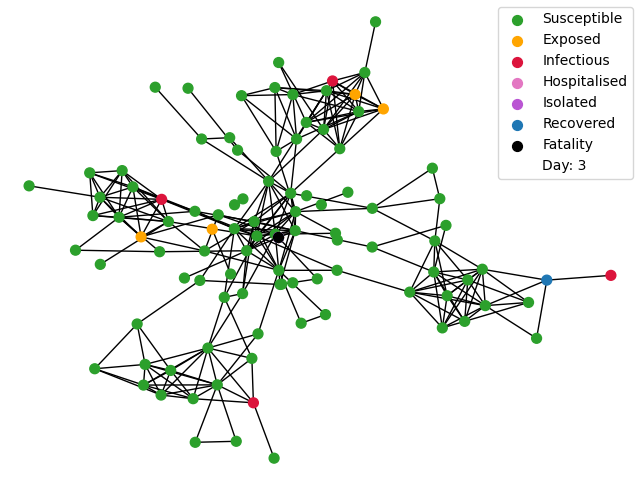
\includegraphics[width=\textwidth]{network}

Example of the network of 100 agents
To simulate the childcare scenario they are split into 5 groups of about 20 agents each with high connectivity inside the group and low connectivity between the groups 
The agents current state is shown by the nodes colour and the edges are that agents close contacts which the disease can spread easiest though the population


\section{Description of Model Parameters}
The Current Modifications of the model relate to allowing 10 of the Model Parameters that relate to Compliance to be dynamically updated each day dependent on a given rule. The 5 most relevent of these being.
\begin{itemize}
\item TESTING\_COMPLIANCE\_RATE\_SYMPTOMATIC (what proportion of agents take a test immediately as a result of having symptoms)
\item TESTING\_COMPLIANCE\_RATE\_RANDOM  (what proportion of agents will do surveillance)
\item ISOLATION\_COMPLIANCE\_RATE\_SYMPTOMATIC\_INDIVIDUAL (what proportion of agents will isolate given they have a symptomatic case)
\item ISOLATION\_COMPLIANCE\_RATE\_POSITIVE\_INDIVIDUAL (what proportion of agents will isolate given a positive result from a test)
\item ISOLATION\_COMPLIANCE\_RATE\_POSITIVE\_GROUPMATE (what proportion of agents in a group isolate given one of them has a positive result from a test)
\end{itemize}

A simple model might only use a few of these compliance parameters such as  and is how the parameters work in the base model
\begin{itemize}
\item TESTING\_COMPLIANCE\_RATE\_SYMPTOMATIC = 0.5\
\item TESTING\_COMPLIANCE\_RATE\_RANDOM = 0.5
\item ISOLATION\_COMPLIANCE\_RATE\_POSITIVE\_INDIVIDUAL =1
\end{itemize}


\section{How to Judge The Effect Parameters Have on A Model?}
On average, what percentage of the population caught the contagion
On average, how many days did it take for the outbreak to stop with 0 active cases

\section{Analysis of Testing Compliance}
We can analyse compliance by comparing the effect varying levels have on the length a contagion actively spreads and what proportion of the population becomes infected. Firstly a baseline can be set to explore the parameter space, then further tests done to see the effect having compliance change as a result of the current known spread of the contagion in the network.


\section{Childcare Model}

\begin{itemize}

\item Parameter justification
\item test false negative rate 0.36 https://www.abc.net.au/news/2022-02-05/staff-children-preschool-childcare-protected-covid-national-plan/100805610
\item R0 mean of Omicron is 9.5, delta is 5.4  https://www1.racgp.org.au/newsgp/clinical/what-to-expect-from-a-third-omicron-wave-in-austra https://academic.oup.com/jtm/article/29/3/taac037/6545354
\item base compliance for behaviour is set t 0.5
\item 100 agents in model split into 5 groups with high interconnectedness within the group and low connections between groups

\item compliance increases for 2 actions,  symtomatic test and regular interva survillencel tests
\item The cost of compliance is is fixed and there is a reward based on if connecting agents are isolated, hospitalised or a fatality

\item from looking at early results since only 2-3 tests a week there is a delay and the higher the r0 the fewer chances they can have to change their mind about compliance 

\item the R0 of 9.5 or 5.4 may be too high as it assumes children spread the disease at the same rate as the general population as well as all disease spread occuring in childcare which it probably is not. Therefore 2 other R0 cases of 3 and 2 are used 
\end{itemize}

\section{Non-Strategic Model}
We have a fixed cost of compliance to an action and varying factors that can raise it. A mix of global and local behavioural factors can be added to make an agent more compliant. In the current build these are the known positive cases in the network in the past 14 days. The proportion of contact agents (those which share an edge) which are a fatality, hospitalised or in isolation. These values are taken away from the base cost and if the result is lower from a specified value the agent will be compliant to that action, otherwise they are not

For a simple example we have a situation for this central agent 

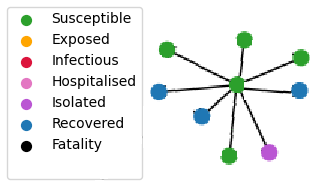
\includegraphics[width=\textwidth]{basicnet}

TESTING\_COMPLIANCE\_RATE\_SYMPTOMATIC                  = 0.5
TESTING\_COMPLIANCE\_RATE\_RANDOM                       = 0.5

14 day positive test rate for network = 0.02 = 2%
This agent’s base aptitude +0.30 which can range (-0.5,0.5)
Base cost = 0.5
Compliance = 0.5 – (5 * 1/10) – (4*0.02) + 0.3 = 0.22
In this case the agent is compliant
will test if they develop a symptomatic case immediately
will do surveillance testing 
if the neighbouring agent that entered hospital returns a positive test, our agent will enter isolation

the reward for agents can be based on a mix of both a local and global network situation as in the example runs

Of the 10 possible compliance parameters built into the existing mode, 4 are used these are,
•	immediately testing if the agent has a symptomatic case
•	using regular surveillance testing
•	isolating if a positive test is returned

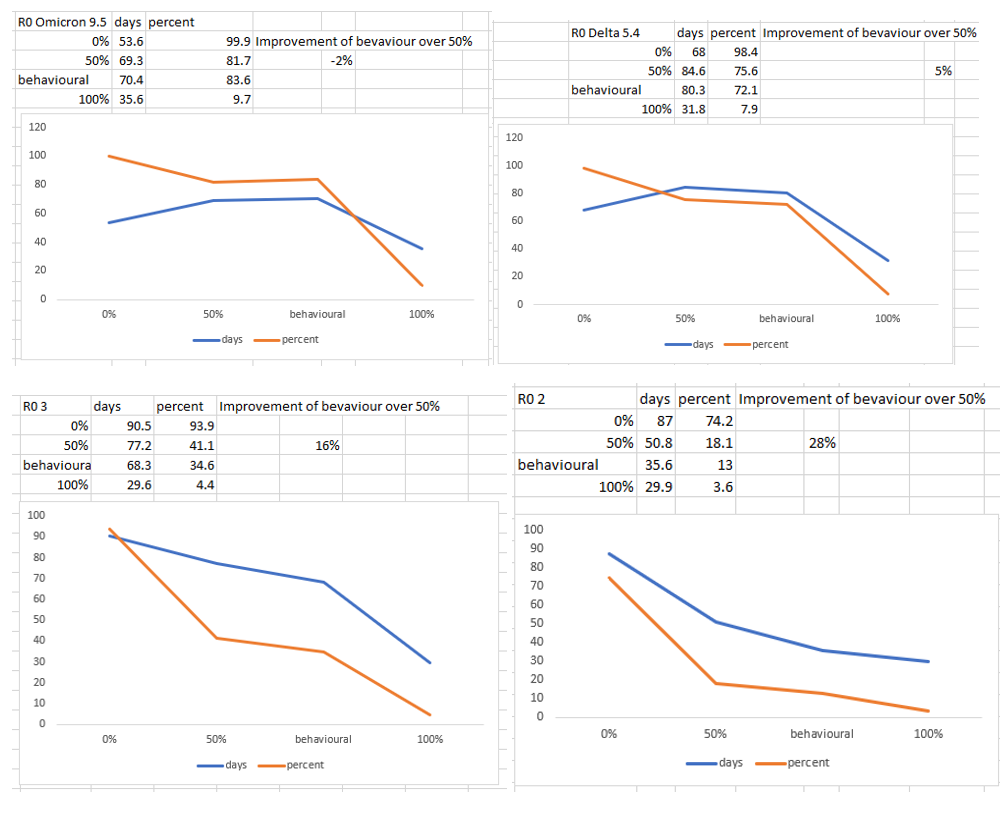
\includegraphics[width=\textwidth]{basicgraph}


Over 3 R0 virus base reproduction rate was the model run with the most important find being the non-strategic behavioural model providing the most improvement over a base static level of compliance as the R0 is reduced, from a -2\% improvement with an R0 of 9.5 to a 28\% improvement with an R0 of 2. This is probably due to one of the aspects the model relating to the 14 day known positive cases recorded. With a low R0 in the system there are more chances for agents to test themselves before they pass on the disease and these reported cases incentivise even more agents to do symptomatic and surveillance testing. With extremely high R0 numbers it is observed that the non-strategic behavioural model has little effect on the total number infected. Across all cases it can be seen that the amount of time the simulation runs for is tied with how many agents get infected. Both the static values of compliance and non-strategic behavioural model follow this trend. 



\section{Strategic Model}


\newpage
\appendix

\section{Appendix Section}

Removed parameter section
\begin{itemize}
\item TRACING\_COMPLIANCE\_RATE (what proportion of agents comply with contact tracing)
\item ISOLATION\_COMPLIANCE\_RATE\_POSITIVE\_CONTACT (what proportion of agents isolate given they are a close contact) 

\item TESTING\_COMPLIANCE\_RATE\_TRACED (what proportion of agents take a test immediately as a result of being informed they are a close contact)


\item ISOLATION\_COMPLIANCE\_RATE\_SYMPTOMATIC\_GROUPMATE (what proportion of agents will isolate given one of their group mates has a symptomatic case)

\item ISOLATION\_COMPLIANCE\_RATE\_POSITIVE\_CONTACTGROUPMATE (what proportion of agents in a group isolate given one of them is a close contact)
\end{itemize}

\end{document}
